% arara: pdflatex: { draft: yes, shell: yes, options: [--output-directory=build] }

% arara: biber: { options: [ '--output-directory=build' ] }
% arara: --> if missing(toFile('build/report.bbl')) || changed(toFile('build/report.bbl')) || found(toFile('build/report.log'), 'Citation')

%! arara: makeglossaries: { options: [ '-d', 'build' ] }
%! arara: --> if changed (toFile('build/report.glo')) || missing (toFile('build/report.gls'))

% arara: pdflatex: { shell: yes, synctex: yes, options: [--output-directory=build] }

% arara: copy: { files: [ 'build/report.pdf' ],
% arara: --> target: 'backup/report.pdf' }

\documentclass{article}

\usepackage{report.preamble}

\begin{document}
    % title
    \title{Introduction to Parallel Computing\\%
    Homework 1: Implicit parallelism techniques and performance
    models.\\%
    \textbf{Results report}%
    }
    \author{Alessandro Iepure}
    \date{25 October 2023}
    \maketitle

    % abstract
    \begin{center}
        \textbf{Abstract}
    \end{center}
    This document analyzes the results and methodologies used while working on the assignment in the title. All work is %
    original and done without input from outside sources except where explicitly noted.
    
    % content
    \section{Array addition and vectorization}

\textit{Task1} and \textit{Task2} ask for two functions, \texttt{routine1()} and \texttt{routine2()} respectively, to %
compute the element-wise sum of two float arrays, namely $a$ and $b$, into another array $c$. Both functions should also %
measure the time it takes the \texttt{for}-loop to complete. \\
The only difference between the two functions is that \texttt{routine2()} uses implicit parallelism. The actual %
logic remains the same. To avoid code duplication, I reused \texttt{routine1()} for both tasks and played with the compiler %
flags to achieve implicit parallelism.\\%
Source code \ref{code:array} shows the trivial implementation of the requested logic.\\
\begin{code}
    \captionof{listing}{\label{code:array}Implemented algorithm}
    \begin{minted}{c}
#include <time.h>

float *routine1(const float *a, const float *b, float *c, int dim) {

    clock_t t0, t1;

    t0 = clock();
    for (int i = 0; i < dim; i++) {
        c[i] = a[i] + b[i];
    }
    t1 = clock();

    printf("%i,%12.4f\n", dim, (t1 - t0) / 1000000.0);
    return c;
}
    \end{minted}
\end{code}
%

After reading GCC's documentation\cite{GCC_vectorization, GCC_dev_opts, GCC_optimize_opts, GCC_x86_opts}, I decided %
to use the following commands to compile the code:
\begin{itemize}
    \item \textit{Task1} (Sequential version): \texttt{gcc -std=c99 -o bin/array-seq.out src/array.c}\\
        Arguments:
        \begin{itemize}
            \item[$\ast$] \texttt{-std=c99}: specifies the \textit{C} dialect used, \textit{C99} in this case. Needed to %
            allow index declarations inside \texttt{for}-loops. It does not impact speed and binary size whatsoever.
            \item[$\ast$] \texttt{-o bin/array-seq.out}: specifies the generated binary file path.
        \end{itemize}
    \item \textit{Task2} (Parallel version): \texttt{gcc -std=c99 -O2 -ftree-vectorize -funroll-loops %
        -fprefetch-loop-arrays -march=native -o bin/array-par.out src/array.c}\\
        Arguments:
        \begin{itemize}
            \item[$\ast$] \texttt{-std=c99}: specifies the \textit{C} dialect used, \textit{C99} in this case. Needed to %
            allow index declarations inside \texttt{for}-loops. It does not impact speed and binary size whatsoever.
            \item[$\ast$] \texttt{-O2}: applies general optimizations that do not involve a space-speed tradeoff%
                \cite{GCC_optimize_opts}
            \item[$\ast$] \texttt{-ftree-vectorize}: enables vectorization\cite{GCC_optimize_opts}
            \item[$\ast$] \texttt{-funroll-loops}: enables loop unrolling\cite{GCC_optimize_opts}
            \item[$\ast$] \texttt{-fprefetch-loop-arrays}: enables memory prefetching to aid looping on large arrays%
                \cite{GCC_optimize_opts}
            \item[$\ast$] \texttt{-march=native}: enables all supported extensions by the CPU in use\footnote{Useful %
                only if the compiling machine is the same as the executing one\cite{GCC_x86_opts}.}. It accelerates mathematical %
                operations, specifically floating-point ones, in hardware\cite{GCC_x86_opts}.
        \end{itemize}
\end{itemize}

The compilation flags, specifically those for the second version, were chosen after testing with multiple combinations. %
After weighting the obtained results, I decided to use the one that yielded a result correctly parallelized and had a visible %
increase in execution speed.\\
Alongside the plain \textit{C} code, I wrote a \textit{bash} script that wraps the compilation commands and binary execution %
into a single file to ease the testing phase. Each binary is called with array sizes between $2^4$ and $2^{22}$ (both inclusive) %
three times. Both sequential and parallelized runs dump their results into a \texttt{CSV} file so that I can examine %
them in external programs.%

\subsection*{Results analysis}
As per indication in the assignment, I executed the script on the University's cluster (GCC 4.3). Table %
\ref{table:array_seq_cluster} and Table \ref{table:array_par_cluster} report the obtained results.%

\begin{table}[h!tb]
    \centering
    \parbox{.45\linewidth}{
        \centering
\caption{Run times by array size - Sequential (times in seconds)}
\begin{tabular}{@{} c c c c c @{}}
\toprule
    \textbf{Size} & \textbf{Run 1}& \textbf{Run 2}& \textbf{Run 3}& \textbf{Average}\\
\midrule
    $2^4$ & 0.0000 & 0.0000 & 0.0000 & 0.0000\\
\lightrule
    $2^5$ & 0.0000 & 0.0000 & 0.0000 & 0.0000\\
\lightrule
    $2^6$ & 0.0000 & 0.0000 & 0.0000 & 0.0000\\
\lightrule
    $2^7$ & 0.0000 & 0.0000 & 0.0000 & 0.0000\\
\lightrule
    $2^8$ & 0.0000 & 0.0000 & 0.0000 & 0.0000\\
\lightrule
    $2^9$ & 0.0000 & 0.0000 & 0.0000 & 0.0000\\
\lightrule
    $2^{10}$ & 0.0000 & 0.0000 & 0.0000 & 0.0000\\
\lightrule
    $2^{11}$ & 0.0000 & 0.0000 & 0.0000 & 0.0000\\
\lightrule
    $2^{12}$ & 0.0000 & 0.0000 & 0.0000 & 0.0000\\
\lightrule
    $2^{13}$ & 0.0000 & 0.0000 & 0.0000 & 0.0000\\
\lightrule
    $2^{14}$ & 0.0000 & 0.0000 & 0.0000 & 0.0000\\
\lightrule
    $2^{15}$ & 0.0000 & 0.0000 & 0.0000 & 0.0000\\
\lightrule
    $2^{16}$ & 0.0000 & 0.0000 & 0.0000 & 0.0000\\
\lightrule
    $2^{17}$ & 0.0000 & 0.0000 & 0.0000 & 0.0000\\
\lightrule
    $2^{18}$ & 0.0000 & 0.0000 & 0.0000 & 0.0000\\
\lightrule
    $2^{19}$ & 0.0000 & 0.0000 & 0.0000 & 0.0000\\
\lightrule
    $2^{20}$ & 0.0200 & 0.0000 & 0.0200 & 0.0133\\
\lightrule
    $2^{21}$ & 0.0200 & 0.0000 & 0.0200 & 0.0133\\
\lightrule
    $2^{22}$ & 0.0200 & 0.0300 & 0.0300 & 0.0267\\
\bottomrule
\end{tabular}
\label{table:array_seq_cluster}
%
    }
    \parbox{.50\linewidth}{
        \centering
\caption{Run times by array size - Parallelised (times in seconds)}
\begin{tabular}{@{} c c c c c @{}}
\toprule
    \textbf{Size} & \textbf{Run 1}& \textbf{Run 2}& \textbf{Run 3}& \textbf{Average}\\
\midrule
    $2^4$ & 0.0000 & 0.0000 & 0.0000 & 0.0000\\
\lightrule
    $2^5$ & 0.0000 & 0.0000 & 0.0000 & 0.0000\\
\lightrule
    $2^6$ & 0.0000 & 0.0000 & 0.0000 & 0.0000\\
\lightrule
    $2^7$ & 0.0000 & 0.0000 & 0.0000 & 0.0000\\
\lightrule
    $2^8$ & 0.0000 & 0.0000 & 0.0000 & 0.0000\\
\lightrule
    $2^9$ & 0.0000 & 0.0000 & 0.0000 & 0.0000\\
\lightrule
    $2^{10}$ & 0.0000 & 0.0000 & 0.0000 & 0.0000\\
\lightrule
    $2^{11}$ & 0.0000 & 0.0000 & 0.0000 & 0.0000\\
\lightrule
    $2^{12}$ & 0.0000 & 0.0000 & 0.0000 & 0.0000\\
\lightrule
    $2^{13}$ & 0.0000 & 0.0000 & 0.0000 & 0.0000\\
\lightrule
    $2^{14}$ & 0.0000 & 0.0000 & 0.0000 & 0.0000\\
\lightrule
    $2^{15}$ & 0.0000 & 0.0000 & 0.0000 & 0.0000\\
\lightrule
    $2^{16}$ & 0.0000 & 0.0000 & 0.0000 & 0.0000\\
\lightrule
    $2^{17}$ & 0.0000 & 0.0000 & 0.0000 & 0.0000\\
\lightrule
    $2^{18}$ & 0.0000 & 0.0000 & 0.0000 & 0.0000\\
\lightrule
    $2^{19}$ & 0.0000 & 0.0000 & 0.0000 & 0.0000\\
\lightrule
    $2^{20}$ & 0.0100 & 0.0000 & 0.0100 & 0.0067\\
\lightrule
    $2^{21}$ & 0.0100 & 0.0100 & 0.0100 & 0.0100\\
\lightrule
    $2^{22}$ & 0.0100 & 0.0200 & 0.0100 & 0.0133\\
\bottomrule
\end{tabular}
\label{table:array_par_cluster}
%
    }
\end{table}

As is visible, the results are mostly instantaneous. Because zero values do not help in weighting the benefits of %
one version over the other, I opted to run the same script on my local machine, a laptop equipped with an Intel%
\textsuperscript{\textregistered} Core\textsuperscript{\texttrademark} i5-8300H at 2.30GHz and 16GB of RAM running Fedora %
38 (GCC 13.2). Table \ref{table:array_seq_local} and Table \ref{table:array_par_local} gather the obtained results.

\begin{table}[h!tb]
    \centering
    \parbox{.45\linewidth}{
        \centering
\caption{Run times by array size - Local machine - Sequential (times in seconds)}
\begin{tabular}{@{} c c c c c @{}}
\toprule
    \textbf{Size} & \textbf{Run 1}& \textbf{Run 2}& \textbf{Run 3}& \textbf{Average}\\
\midrule
    $2^4$ & 0.0000 & 0.0000 & 0.0000 & 0.0000\\
\lightrule
    $2^5$ & 0.0000 & 0.0000 & 0.0000 & 0.0000\\
\lightrule
    $2^6$ & 0.0000 & 0.0000 & 0.0000 & 0.0000\\
\lightrule
    $2^7$ & 0.0000 & 0.0000 & 0.0000 & 0.0000\\
\lightrule
    $2^8$ & 0.0000 & 0.0000 & 0.0000 & 0.0000\\
\lightrule
    $2^9$ & 0.0000 & 0.0000 & 0.0000 & 0.0000\\
\lightrule
    $2^{10}$ & 0.0000 & 0.0000 & 0.0000 & 0.0000\\
\lightrule
    $2^{11}$ & 0.0000 & 0.0000 & 0.0000 & 0.0000\\
\lightrule
    $2^{12}$ & 0.0000 & 0.0000 & 0.0000 & 0.0000\\
\lightrule
    $2^{13}$ & 0.0000 & 0.0000 & 0.0000 & 0.0000\\
\lightrule
    $2^{14}$ & 0.0001 & 0.0001 & 0.0001 & 0.0001\\
\lightrule
    $2^{15}$ & 0.0001 & 0.0001 & 0.0001 & 0.0001\\
\lightrule
    $2^{16}$ & 0.0003 & 0.0003 & 0.0002 & 0.0003\\
\lightrule
    $2^{17}$ & 0.0005 & 0.0005 & 0.0006 & 0.0005\\
\lightrule
    $2^{18}$ & 0.0010 & 0.0012 & 0.0010 & 0.0011\\
\lightrule
    $2^{19}$ & 0.0021 & 0.0021 & 0.0023 & 0.0022\\
\lightrule
    $2^{20}$ & 0.0041 & 0.0041 & 0.0041 & 0.0041\\
\lightrule
    $2^{21}$ & 0.0082 & 0.0081 & 0.0081 & 0.0081\\
\lightrule
    $2^{22}$ & 0.0163 & 0.0160 & 0.0161 & 0.0161\\
\bottomrule
\end{tabular}
\label{table:array_seq_local}
%
    }
    \parbox{.50\linewidth}{
        \centering
\caption{Run times by array size - Local machine - Parallelised (times in seconds)}
\begin{tabular}{@{} c c c c c @{}}
\toprule
    \textbf{Size} & \textbf{Run 1}& \textbf{Run 2}& \textbf{Run 3}& \textbf{Average}\\
\midrule
    $2^4$ & 0.0000 & 0.0000 & 0.0000 & 0.0000\\
\lightrule
    $2^5$ & 0.0000 & 0.0000 & 0.0000 & 0.0000\\
\lightrule
    $2^6$ & 0.0000 & 0.0000 & 0.0000 & 0.0000\\
\lightrule
    $2^7$ & 0.0000 & 0.0000 & 0.0000 & 0.0000\\
\lightrule
    $2^8$ & 0.0000 & 0.0000 & 0.0000 & 0.0000\\
\lightrule
    $2^9$ & 0.0000 & 0.0000 & 0.0000 & 0.0000\\
\lightrule
    $2^{10}$ & 0.0000 & 0.0000 & 0.0000 & 0.0000\\
\lightrule
    $2^{11}$ & 0.0000 & 0.0000 & 0.0000 & 0.0000\\
\lightrule
    $2^{12}$ & 0.0000 & 0.0000 & 0.0000 & 0.0000\\
\lightrule
    $2^{13}$ & 0.0000 & 0.0000 & 0.0000 & 0.0000\\
\lightrule
    $2^{14}$ & 0.0000 & 0.0000 & 0.0000 & 0.0000\\
\lightrule
    $2^{15}$ & 0.0001 & 0.0001 & 0.0001 & 0.0001\\
\lightrule
    $2^{16}$ & 0.0001 & 0.0001 & 0.0001 & 0.0001\\
\lightrule
    $2^{17}$ & 0.0003 & 0.0002 & 0.0002 & 0.0002\\
\lightrule
    $2^{18}$ & 0.0005 & 0.0006 & 0.0005 & 0.0005\\
\lightrule
    $2^{19}$ & 0.0009 & 0.0009 & 0.0009 & 0.0009\\
\lightrule
    $2^{20}$ & 0.0018 & 0.0018 & 0.0017 & 0.0018\\
\lightrule
    $2^{21}$ & 0.0036 & 0.0036 & 0.0036 & 0.0036\\
\lightrule
    $2^{22}$ & 0.0073 & 0.0082 & 0.0096 & 0.0084\\
\bottomrule
\end{tabular}
\label{table:array_par_local}
%
    }
\end{table}

Results from different machines with different architectures and components cannot be compared top each other, especially %
if the code is compiled for a particular machine. From now on, I am going to consider only the results obtained from my laptop.\\%
The average run times are plotted in Plot \ref{plot:array}. The obtained graph is the initial part of the so-called %
\textquote{Roofline model}. If the program were to be run with higher values and the machine was able to compute the result, 
the graph would rise to a certain point called \textquote{peak} and from then on would continue as a flat line having reached %
the maximum performance.\\%
Overall, by implicitly parallelizing the code, we gained around 57\% (average) more execution speed.%
\begin{code}
    \captionof{listing}{\label{code:array}Implemented algorithm}
    \begin{minted}{c}
#include <time.h>

float *routine1(const float *a, const float *b, float *c, int dim) {

    clock_t t0, t1;

    t0 = clock();
    for (int i = 0; i < dim; i++) {
        c[i] = a[i] + b[i];
    }
    t1 = clock();

    printf("%i,%12.4f\n", dim, (t1 - t0) / 1000000.0);
    return c;
}
    \end{minted}
\end{code}

    \clearpage
    \section{Matrix copy via block reverse ordering}
\textit{Task1} and \textit{Task2} ask for two functions, \texttt{routine1()} and \texttt{routine2()} respectively, that %
take a matrix $M$ of size $N\times N$ and reverse the order in blocks $b\times b$ in another matrix $O$.\\%
As the previous exercise, the only difference between the two functions is whether implicit parallelism is used. I chose %
again to avoid code duplication and accomplish what was requested via compilation flags, the same used in the previous %
exercise. In addition, the \textit{bash} script was integrated with the new commands and, as before, each version was %
executed three times with $b$ values ranging from $2^2$ to $2^8$ (inclusive).\\%
Source code \ref{code:matrix} shows the implemented algorithm. It loops around each $b\times b$ block in the original %
matrix $M$ and, for each, copies the values of the current block and the opposite one in the reverse order. Doing both %
copies in the same iteration allows the main matrix to be looped only for half of the rows.
\begin{figure}[h!tb]
    \centering
    \captionsetup{type=plot}
    \caption{\label{plot:matrix}Effective bandwidth by $b$ size}
    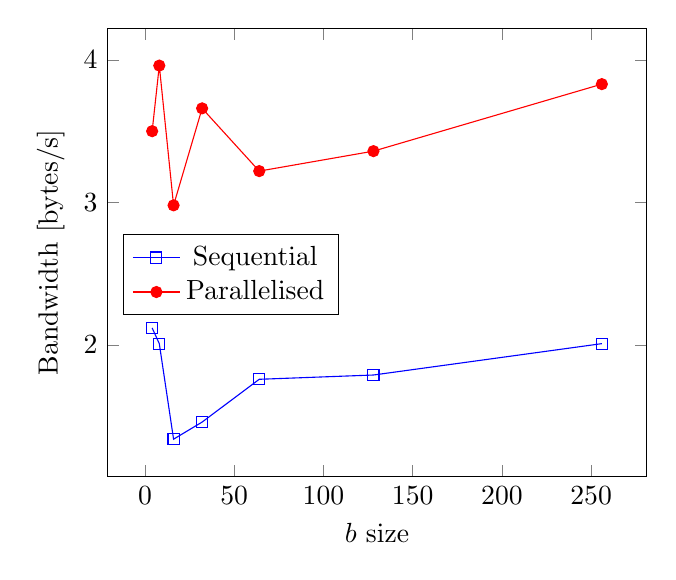
\begin{tikzpicture}
        \begin{axis}[
            title={},
            xlabel={$b$ size},
            ylabel={Bandwidth [bytes/s]},
            legend style={at={(0.03,0.45)},anchor=west}
        ]
            \addplot[
                color=blue,
                mark=square,
                ]
                coordinates {
                    (4,2.12)
                    (8,2.01)
                    (16,1.34)
                    (32,1.46)
                    (64,1.76)
                    (128,1.79)
                    (256,2.01)
                };
            
            \addplot[
                color=red,
                mark=*,
                ]
                coordinates {
                    (4,3.50)
                    (8,3.96)
                    (16,2.98)
                    (32,3.66)
                    (64,3.22)
                    (128,3.36)
                    (256,3.83)
                };
            \legend{Sequential, Parallelised}
        \end{axis}
    \end{tikzpicture}
\end{figure}

\subsection*{Results analysis}
Table \ref{table:matrix_seq} and Table \ref{table:matrix_par} show the run times obtained for each execution. The parallel %
version is 49\% (average) quicker than the same algorithm executed sequentialy.%

\begin{table}[h!tb]
    \centering
    \parbox{.45\linewidth}{
        \centering
\caption{\label{table:matrix_seq}Run times by $b$ size - Sequential (times in seconds)}
\begin{tabular}{@{} c c c c c @{}}
\toprule
    \textbf{Size} & \textbf{Run 1}& \textbf{Run 2}& \textbf{Run 3}& \textbf{Average}\\
\midrule
    $2^2$ & 0.1200 & 0.1300 & 0.1300 & 0.1267\\
\lightrule
    $2^3$ & 0.1400 & 0.1400 & 0.1200 & 0.1333\\
\lightrule
    $2^4$ & 0.2000 & 0.2000 & 0.2000 & 0.2000\\
\lightrule
    $2^5$ & 0.1900 & 0.1700 & 0.1800 & 0.1800\\
\lightrule
    $2^6$ & 0.1600 & 0.1600 & 0.1600 & 0.1600\\
\lightrule
    $2^7$ & 0.1500 & 0.1500 & 0.1500 & 0.1500\\
\lightrule
    $2^8$ & 0.1400 & 0.1300 & 0.1300 & 0.1333\\
\bottomrule
\end{tabular}
%
    }
    \parbox{.50\linewidth}{
        \centering
\caption{\label{table:matrix_par}Run times by $b$ size - Parallelised (times in seconds)}
\begin{tabular}{@{} c c c c c @{}}
\toprule
    \textbf{Size} & \textbf{Run 1}& \textbf{Run 2}& \textbf{Run 3}& \textbf{Average}\\
\midrule
    $2^2$ & 0.0700 & 0.0800 & 0.0800 & 0.0767\\
\lightrule
    $2^3$ & 0.0700 & 0.0600 & 0.0700 & 0.0667\\
\lightrule
    $2^4$ & 0.0800 & 0.1000 & 0.0900 & 0.0900\\
\lightrule
    $2^5$ & 0.0800 & 0.0700 & 0.0700 & 0.0733\\
\lightrule
    $2^6$ & 0.0800 & 0.0900 & 0.0800 & 0.0833\\
\lightrule
    $2^7$ & 0.0700 & 0.0900 & 0.0800 & 0.0800\\
\lightrule
    $2^8$ & 0.0700 & 0.0700 & 0.0700 & 0.0700\\
\bottomrule
\end{tabular}
%
    }
\end{table}

To compute the effective bandwidth, it is necessary to know the number of bytes read $B_r$ and written $B_w$. In our %
case, both values are equal and calculated as $(N\times N) * S_f$, where $N\times N$ is the size of the matrix $M$ and %
$S_f$ is the size of a \textit{float} type (4 bytes). The algorithm reads two values and stores the same %
quantity, totaling four operations for each matrix position. Substituting this information in equation (\ref{eq:bandwidth}), %
we get the results in Table \ref{table:bandwidths}. Plot \ref{plot:matrix} shows a visual representation of the effective %
bandwidth.

\begin{equation}
    \label{eq:bandwidth}
    b=\frac{(B_r+B_w)/10^9}{t}=\frac{(4*4096^2*4)/10^9}{t}\qquad[\textnormal{GB/s}]
\end{equation}

\begin{table}[h!tb]
    \centering
    \caption{\label{table:bandwidths}Effective bandwidths in GB/s}
    \begin{tabular}{@{} c c c @{}}
    \toprule
        \textbf{Size} & \textbf{Sequential}& \textbf{Parallelised}\\
    \midrule
        $2^2$ & 2.12 & 3.50\\
    \lightrule
        $2^3$ & 2.01 & 3.96\\
    \lightrule
        $2^4$ & 1.34 & 2.98\\
    \lightrule
        $2^5$ & 1.49 & 3.66\\
    \lightrule
        $2^6$ & 1.76 & 3.22\\
    \lightrule
        $2^7$ & 1.79 & 3.36\\
    \lightrule
        $2^8$ & 2.01 & 3.83 \\
    \midrule
        Average & 1.79 & 3.50\\
    \bottomrule
    \end{tabular}
\end{table}
\begin{figure}[h!tb]
    \centering
    \captionsetup{type=plot}
    \caption{\label{plot:matrix}Effective bandwidth by $b$ size}
    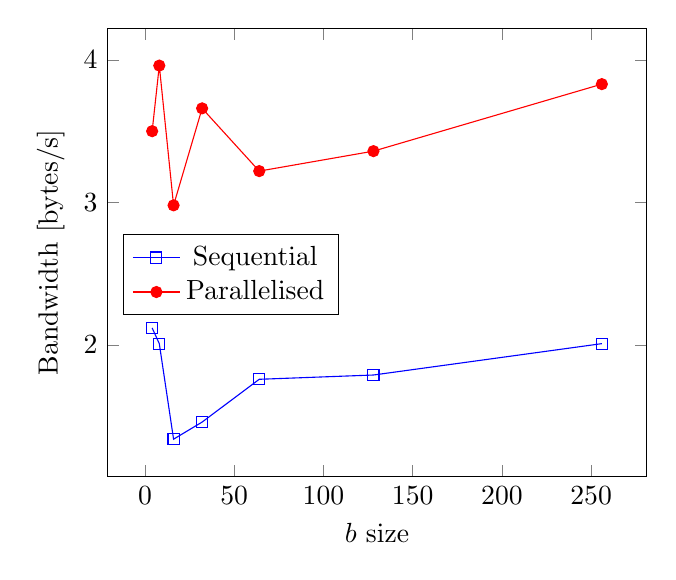
\begin{tikzpicture}
        \begin{axis}[
            title={},
            xlabel={$b$ size},
            ylabel={Bandwidth [bytes/s]},
            legend style={at={(0.03,0.45)},anchor=west}
        ]
            \addplot[
                color=blue,
                mark=square,
                ]
                coordinates {
                    (4,2.12)
                    (8,2.01)
                    (16,1.34)
                    (32,1.46)
                    (64,1.76)
                    (128,1.79)
                    (256,2.01)
                };
            
            \addplot[
                color=red,
                mark=*,
                ]
                coordinates {
                    (4,3.50)
                    (8,3.96)
                    (16,2.98)
                    (32,3.66)
                    (64,3.22)
                    (128,3.36)
                    (256,3.83)
                };
            \legend{Sequential, Parallelised}
        \end{axis}
    \end{tikzpicture}
\end{figure}

    \clearpage
    \printbibliography
\end{document}